
\section{\rqtwo}
\label{rq2:method}

In this second research question, we investigate to what extent the artificially created variants are dynamically different between them and to the original program. To conduct this research question, we could separate the question in three fields as \autoref{diagrams:protocol:rq2} illustrates: static comparison, variant's preservation and  dynamic comparison. %The three fields are addressed in the CROW and MEWE contributions.
The static analysis focuses on the appreciated differences between the program variants between them and against the original program, and we address it in the answering of RQ1. The preservation study highlight the fact that \wasm still is an intermediate code and compilers can undo code transformations from previous stages, therefore, it is important to conduct a study on how these transformations are maintained through \wasm programs' lifecycle, from their creation to the machine code execution. The preservation study is out of the scope of this work, and it was previously addressed in CROW and MEWE contributions.
All that said, with RQ2, we focus on the last category, the dynamic analysis of the generated variants. This decision is supported due to that dynamic side-channels are offered through the execution of \wasm and we want to go deeper in this analysis.
We use the original functions from the \corpusrosetta corpus described in \autoref{section:crow:corpora} and their variants generated in the answering of RQ1. 
We use only the \corpusrosetta to answer RQ2 because this corpus is composed by simple programs that can be executed directly without user interaction.

\todo{stress this fact}

\begin{figure*}[h]
    \centering
    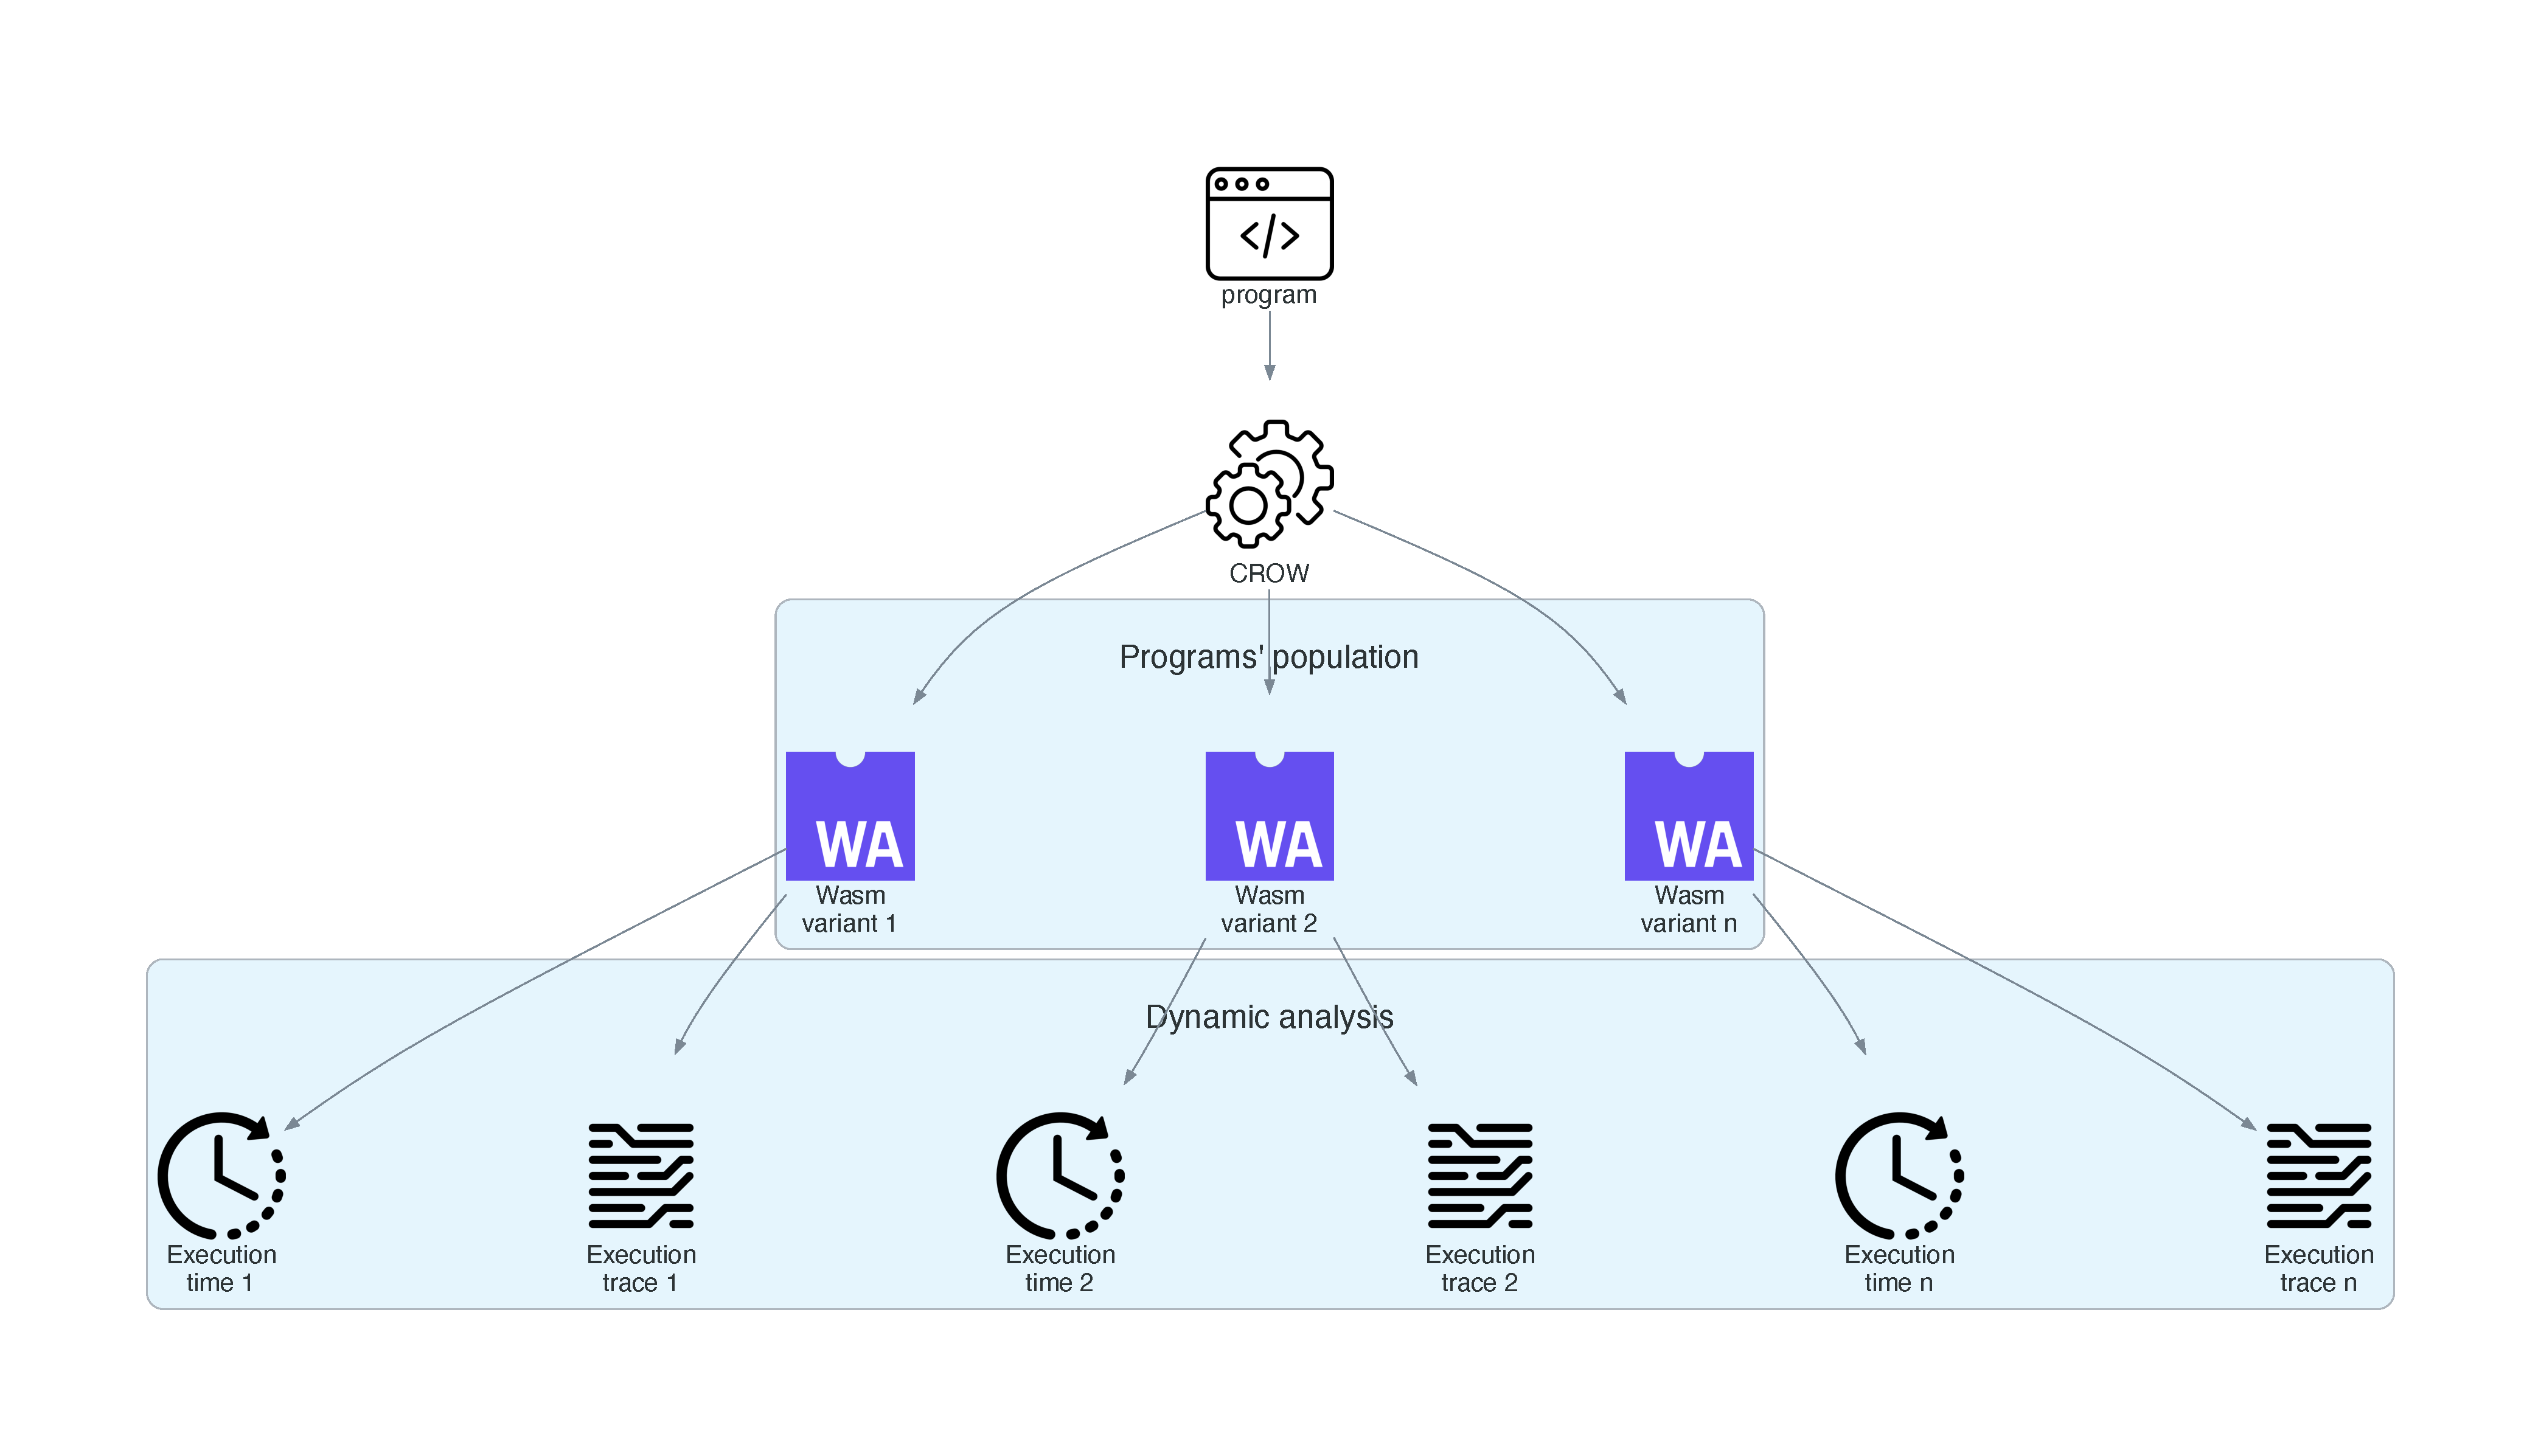
\includegraphics[height=2.8in]{diagrams/Rq2.pdf}
    \caption{Population study methodology for each original corpora and the variants generated in RQ1.}
    \label{diagrams:protocol:rq2}
\end{figure*}

We execute each program on each population of variants to collect their execution traces and execution times. Furthermore, we compare their dynamic behavior. We perform fine-grained comparisons by studying all pairs of programs in the population of variants plus the original program. Therefore, the defined metrics are formulated to support a pairwise comparison strategy.
In the following, we define the metrics used to answer RQ2.

\subsection*{Metrics}

We measure the difference between programs at runtime by comparing their execution times and execution traces. We compare their execution traces with an alignment metric at the function and instruction level. Concretely, we propose a global alignment approach using Dynamic Time Warping (DTW) for their execution traces. %In previous work, we highlighted how this approach measure similarity \citationneeded. 
Dynamic Time Warping \cite{Maia08usinga} computes the global alignment between two sequences. It returns a value capturing the cost of this alignment, which is a distance metric. The larger the DTW distance, the more different the two sequences are.
In the following, we define the $\DTW$ metric. 
 

\begin{metric}{\DTW{}:}
\label{metric:stack}
	Given two programs P and P' from the same program's population, \DTW{}(P,P'), computes the DTW distance between the traces collected during their execution. \\
	A \DTW{} of $0$ means that both traces are identical.
	The higher the value, the more different the traces. 
\end{metric}


In our experiments, a program trace is the consecutive list of \texttt{push} and \texttt{pop} operations performed by the \wasm engine during the execution of the program.

We use the execution time of the programs in the population to complement the answer to RQ2. We compare each execution time distribution from the variants against the distribution of the original program.

\begin{metric}{Execution time:}\label{metric:time}
	Given a \wasm program P, the execution time is the time spent to execute the binary.
\end{metric}

%\subsection{Variants preservation}

\subsection*{Protocol}

% Dynamic
To compare program and variants behavior during runtime, we analyze all the unique program variants generated in the answering of RQ1 in a pairwise comparison using \autoref{metric:stack}. We use SWAM\footnote{\url{https://github.com/satabin/swam}} to execute each program and variant to collect the stack traces in the case of the \corpusrosetta corpus. SWAM is a \wasm interpreter that provides functionalities to capture the dynamic information of \wasm program executions, including the virtual stack operations. 

Furthermore, we collect the execution time, \autoref{metric:time}, for all programs and their variants. We compare the collected execution time distributions between programs using a Mann-Withney test \cite{mann1947} in a pairwise strategy.

\todo{Maybe the first time that Mann-Withney is mentioned I should describe what it is}

 